% GNUPLOT: LaTeX picture with Postscript
\begingroup
  \makeatletter
  \providecommand\color[2][]{%
    \GenericError{(gnuplot) \space\space\space\@spaces}{%
      Package color not loaded in conjunction with
      terminal option `colourtext'%
    }{See the gnuplot documentation for explanation.%
    }{Either use 'blacktext' in gnuplot or load the package
      color.sty in LaTeX.}%
    \renewcommand\color[2][]{}%
  }%
  \providecommand\includegraphics[2][]{%
    \GenericError{(gnuplot) \space\space\space\@spaces}{%
      Package graphicx or graphics not loaded%
    }{See the gnuplot documentation for explanation.%
    }{The gnuplot epslatex terminal needs graphicx.sty or graphics.sty.}%
    \renewcommand\includegraphics[2][]{}%
  }%
  \providecommand\rotatebox[2]{#2}%
  \@ifundefined{ifGPcolor}{%
    \newif\ifGPcolor
    \GPcolorfalse
  }{}%
  \@ifundefined{ifGPblacktext}{%
    \newif\ifGPblacktext
    \GPblacktexttrue
  }{}%
  % define a \g@addto@macro without @ in the name:
  \let\gplgaddtomacro\g@addto@macro
  % define empty templates for all commands taking text:
  \gdef\gplbacktext{}%
  \gdef\gplfronttext{}%
  \makeatother
  \ifGPblacktext
    % no textcolor at all
    \def\colorrgb#1{}%
    \def\colorgray#1{}%
  \else
    % gray or color?
    \ifGPcolor
      \def\colorrgb#1{\color[rgb]{#1}}%
      \def\colorgray#1{\color[gray]{#1}}%
      \expandafter\def\csname LTw\endcsname{\color{white}}%
      \expandafter\def\csname LTb\endcsname{\color{black}}%
      \expandafter\def\csname LTa\endcsname{\color{black}}%
      \expandafter\def\csname LT0\endcsname{\color[rgb]{1,0,0}}%
      \expandafter\def\csname LT1\endcsname{\color[rgb]{0,1,0}}%
      \expandafter\def\csname LT2\endcsname{\color[rgb]{0,0,1}}%
      \expandafter\def\csname LT3\endcsname{\color[rgb]{1,0,1}}%
      \expandafter\def\csname LT4\endcsname{\color[rgb]{0,1,1}}%
      \expandafter\def\csname LT5\endcsname{\color[rgb]{1,1,0}}%
      \expandafter\def\csname LT6\endcsname{\color[rgb]{0,0,0}}%
      \expandafter\def\csname LT7\endcsname{\color[rgb]{1,0.3,0}}%
      \expandafter\def\csname LT8\endcsname{\color[rgb]{0.5,0.5,0.5}}%
    \else
      % gray
      \def\colorrgb#1{\color{black}}%
      \def\colorgray#1{\color[gray]{#1}}%
      \expandafter\def\csname LTw\endcsname{\color{white}}%
      \expandafter\def\csname LTb\endcsname{\color{black}}%
      \expandafter\def\csname LTa\endcsname{\color{black}}%
      \expandafter\def\csname LT0\endcsname{\color{black}}%
      \expandafter\def\csname LT1\endcsname{\color{black}}%
      \expandafter\def\csname LT2\endcsname{\color{black}}%
      \expandafter\def\csname LT3\endcsname{\color{black}}%
      \expandafter\def\csname LT4\endcsname{\color{black}}%
      \expandafter\def\csname LT5\endcsname{\color{black}}%
      \expandafter\def\csname LT6\endcsname{\color{black}}%
      \expandafter\def\csname LT7\endcsname{\color{black}}%
      \expandafter\def\csname LT8\endcsname{\color{black}}%
    \fi
  \fi
    \setlength{\unitlength}{0.0500bp}%
    \ifx\gptboxheight\undefined%
      \newlength{\gptboxheight}%
      \newlength{\gptboxwidth}%
      \newsavebox{\gptboxtext}%
    \fi%
    \setlength{\fboxrule}{0.5pt}%
    \setlength{\fboxsep}{1pt}%
\begin{picture}(7200.00,5040.00)%
    \gplgaddtomacro\gplbacktext{%
      \csname LTb\endcsname%
      \put(165,2646){\makebox(0,0)[r]{\strut{}$-3$}}%
      \put(165,2961){\makebox(0,0)[r]{\strut{}$-2$}}%
      \put(165,3276){\makebox(0,0)[r]{\strut{}$-1$}}%
      \put(165,3591){\makebox(0,0)[r]{\strut{}$0$}}%
      \put(165,3905){\makebox(0,0)[r]{\strut{}$1$}}%
      \put(165,4220){\makebox(0,0)[r]{\strut{}$2$}}%
      \put(165,4535){\makebox(0,0)[r]{\strut{}$3$}}%
      \put(429,2363){\makebox(0,0){\strut{} }}%
      \put(916,2363){\makebox(0,0){\strut{} }}%
      \put(1403,2363){\makebox(0,0){\strut{} }}%
      \put(1890,2363){\makebox(0,0){\strut{} }}%
      \put(2376,2363){\makebox(0,0){\strut{} }}%
      \put(2863,2363){\makebox(0,0){\strut{} }}%
      \put(3350,2363){\makebox(0,0){\strut{} }}%
    }%
    \gplgaddtomacro\gplfronttext{%
      \csname LTb\endcsname%
      \put(-341,3590){\rotatebox{-270}{\makebox(0,0){\strut{}$\varepsilon_k, \Delta_k$}}}%
      \put(833,4378){\makebox(0,0){\strut{}$\nu = 1$}}%
    }%
    \gplgaddtomacro\gplbacktext{%
      \csname LTb\endcsname%
      \put(3584,2646){\makebox(0,0)[r]{\strut{} }}%
      \put(3584,2961){\makebox(0,0)[r]{\strut{} }}%
      \put(3584,3276){\makebox(0,0)[r]{\strut{} }}%
      \put(3584,3591){\makebox(0,0)[r]{\strut{} }}%
      \put(3584,3905){\makebox(0,0)[r]{\strut{} }}%
      \put(3584,4220){\makebox(0,0)[r]{\strut{} }}%
      \put(3584,4535){\makebox(0,0)[r]{\strut{} }}%
      \put(3848,2363){\makebox(0,0){\strut{} }}%
      \put(4335,2363){\makebox(0,0){\strut{} }}%
      \put(4822,2363){\makebox(0,0){\strut{} }}%
      \put(5309,2363){\makebox(0,0){\strut{} }}%
      \put(5796,2363){\makebox(0,0){\strut{} }}%
      \put(6283,2363){\makebox(0,0){\strut{} }}%
      \put(6770,2363){\makebox(0,0){\strut{} }}%
    }%
    \gplgaddtomacro\gplfronttext{%
      \csname LTb\endcsname%
      \put(4253,4378){\makebox(0,0){\strut{}$\nu = 1$}}%
    }%
    \gplgaddtomacro\gplbacktext{%
      \csname LTb\endcsname%
      \put(165,504){\makebox(0,0)[r]{\strut{}$-3$}}%
      \put(165,819){\makebox(0,0)[r]{\strut{}$-2$}}%
      \put(165,1134){\makebox(0,0)[r]{\strut{}$-1$}}%
      \put(165,1449){\makebox(0,0)[r]{\strut{}$0$}}%
      \put(165,1763){\makebox(0,0)[r]{\strut{}$1$}}%
      \put(165,2078){\makebox(0,0)[r]{\strut{}$2$}}%
      \put(165,2393){\makebox(0,0)[r]{\strut{}$3$}}%
      \put(429,221){\makebox(0,0){\strut{}$-3$}}%
      \put(916,221){\makebox(0,0){\strut{}$-2$}}%
      \put(1403,221){\makebox(0,0){\strut{}$-1$}}%
      \put(1890,221){\makebox(0,0){\strut{}$0$}}%
      \put(2376,221){\makebox(0,0){\strut{}$1$}}%
      \put(2863,221){\makebox(0,0){\strut{}$2$}}%
      \put(3350,221){\makebox(0,0){\strut{}$3$}}%
    }%
    \gplgaddtomacro\gplfronttext{%
      \csname LTb\endcsname%
      \put(-209,1448){\rotatebox{-270}{\makebox(0,0){\strut{}$\varepsilon_k, \Delta_k$}}}%
      \put(1889,-109){\makebox(0,0){\strut{}$kd$}}%
      \put(833,2236){\makebox(0,0){\strut{}$\nu = 0$}}%
    }%
    \gplgaddtomacro\gplbacktext{%
      \csname LTb\endcsname%
      \put(3584,504){\makebox(0,0)[r]{\strut{} }}%
      \put(3584,819){\makebox(0,0)[r]{\strut{} }}%
      \put(3584,1134){\makebox(0,0)[r]{\strut{} }}%
      \put(3584,1449){\makebox(0,0)[r]{\strut{} }}%
      \put(3584,1763){\makebox(0,0)[r]{\strut{} }}%
      \put(3584,2078){\makebox(0,0)[r]{\strut{} }}%
      \put(3584,2393){\makebox(0,0)[r]{\strut{} }}%
      \put(3848,221){\makebox(0,0){\strut{}$-3$}}%
      \put(4335,221){\makebox(0,0){\strut{}$-2$}}%
      \put(4822,221){\makebox(0,0){\strut{}$-1$}}%
      \put(5309,221){\makebox(0,0){\strut{}$0$}}%
      \put(5796,221){\makebox(0,0){\strut{}$1$}}%
      \put(6283,221){\makebox(0,0){\strut{}$2$}}%
      \put(6770,221){\makebox(0,0){\strut{}$3$}}%
    }%
    \gplgaddtomacro\gplfronttext{%
      \csname LTb\endcsname%
      \put(5309,-109){\makebox(0,0){\strut{}$kd$}}%
      \put(4253,2236){\makebox(0,0){\strut{}$\nu = 2$}}%
    }%
    \gplbacktext
    \put(0,0){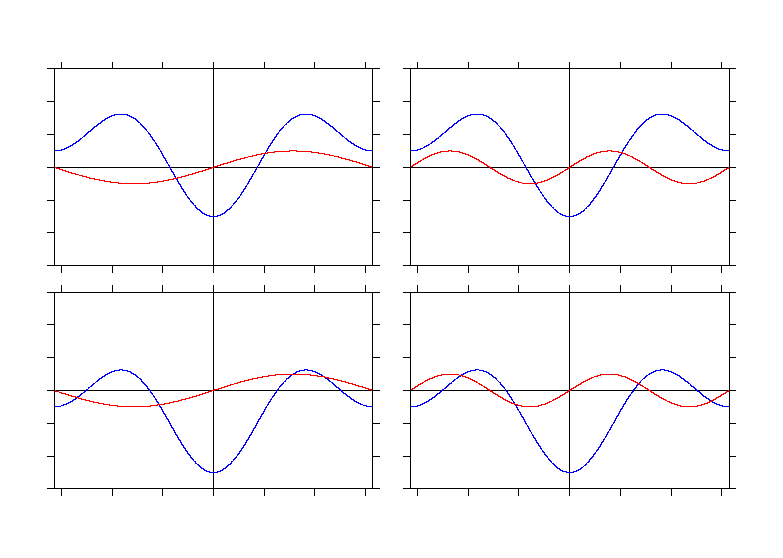
\includegraphics{Figures/Lattice.singlewire/dispersion/kdepend}}%
    \gplfronttext
  \end{picture}%
\endgroup
